\section{ساختار تصویربرداری \mri}\label{sec:mri-basics}

\subsection{تاریخچه}


تاریخچه تصویربرداری تشدید مفناطیسی
\LTRfootnote{Magnetic Resonance Imaging}(\mri)
تلاش تعداد زیادی از محققانی را شامل می‌شود که پدیده تشدید مغناطیسی هسته
\LTRfootnote{Nuclear Magnetic Resonance}(\lr{NMR})
را کشف کردند.
در سال ۱۹۵۰، حصول تصویر یک بعدی \mri توسط هرمن کار 
\LTRfootnote{Herman Carr}
 گزارش گردید. پاول لاتربر 
\LTRfootnote{Paul C. Lauterbur}
، شیمیدان آمریکایی با کار بر روی تحقیقات پیشین، موفق به ابداع روش‌هایی برای تولید تصاویر دو بعدی و سه بعدی \mri گردید. سرانجام وی در سال ۱۹۷۳ اولین تصویر گرفته شده بر اساس تشدید مغناطیس هسته‌ای (\lr{NMR}) خود را منتشر نمود. اولین تصویر مقطع نگاری از یک موش زنده در ژانویه ۱۹۷۴ منتشر گردید.


از سوی دیگر تحقیقات و پیشرفت‌های مهمی در زمینهٔ تصویر برداری بر اساس تشدید مغناطیسی هسته برای نخستین بار در دانشگاه ناتینگهام انگلستان 
\LTRfootnote{University of Nottingham}
صورت پذیرفت، جایی که پیتر منسفیلد فیزیکدان برجستهٔ آن مؤسسه با گسترش یک روش ریاضی موفق به کاهش زمان تصویربرداری و افزایش کیفت تصاویر نسبت به روش بکارگرفته شده توسط لاتربر گردید. در همان زمان در سال ۱۹۷۱ دانشمند آمریکایی ارمنی تبار ریموند دامادیان استاد دانشگاه ایالتی نیویورک در مقاله‌ای که در مجلهٔ Science منتشر گردید، اعلام نمود که امکان تشخیص تومور از بافت‌های عادی به کمک تصویر برداری 
\lr{NMR}
 میسر می‌باشد.

سرانجام جایزهٔ نوبل پزشکی سال ۲۰۰۳ به خاطر اختراع ام آر آی به پاول لاتربر از دانشگاه ایلینوی در اوربانا شامپاین و پیتر منزفیلد از انگلستان اعطا گردید. 
این جایزه به تنهایی می‌تواند اهمیت این نوع تصویربرداری را نشان دهد.

اما چه عواملی باعث شده‌اند تا این‌قدر \mri بااهمیت و ویژه باشند؟ تصویربرداری \mri روشی غیر تهاجمی و نسبتا امن است. 

سیستم‌های ام آر آی امروزه غالباً دارای قدرت میدان‌های ۰/۲، ۱، ۱/۵، و ۳ تسلا می‌باشند.
در ایالات متحده آمریکا بیمارستان‌ها و مراکز خدمات بهداشتی اجازه استفاده از سیستم‌های تا ۴ تسلا را نیز برای یک بیمار دارند. اما از چهار تسلا به بالا صرفاً جنبه و کاربردهای تحقیقاتی دارد.

امروزه بزرگ‌ترین تولیدکننده‌های سیستم‌های ام آر آی شرکت‌های زیمنس (آلمان)، جنرال الکتریک (آمریکا)، توشیبا (ژاپن)، و فیلیپس (هلند) می‌باشند.

\subsection{خطرات \mri}
برخلاف سایر دستگاه‌های تصویربرداری مثل اشعه ایکس و سی‌تی اسکن، ام آر آی از تشعشع یونیزه استفاده نمی‌کند. از این ابزار می‌توان برای تصویربرداری از جنین در دوران بارداری استفاده کرد بدون آن که اثری روی آن داشته باشد. اما باز هم این روش ممکن است خطراتی در پی داشته باشد و به همین دلیل جوامع پزشکی استفاده از \mri را در مراحل اولیه تشخیص بیماری توصیه نمی‌کنند. از آن‌جایی که در فرآیند ام آر آی از مغناطیس قوی استفاده می‌شود هر قطعه فلزی که در بدن وجود داشته باشد مثل ضربان ساز قلب، مفصل مصنوعی، دریچه مصنوعی قلب، حلزون مصنوعی گوش و یا هر نوع صفحه و پیچ و مهره فلزی در بدن ممکن است خطرساز باشد، چون میدان مغناطیسی می‌تواند باعث جابجایی و یا گرم شدن آن قطعه شود.

تعدادی از بیمارانی که از ضربان ساز قلب استفاده می‌کردند طی انجام ام آر آی از دنیا رفتند. بنابراین لازم است تکنولوژیست \mri سوالات لازم را قبل از انجام این فرآیند از بیمار بپرسد. البته بیشتر قطعات فلزی که امروز در ایمپلنت‌های بدن استفاده قرار می‌شوند تحت تأثیر میدان‌های مغناطیسی قرار نمی‌گیرند و به اصطلاح
\lr{MR-Safe}
 هستند. علاوه بر این، هنگام اسکن، دستگاه ام آر آی صداهای بلندی تولید می‌کند که ممکن است باعث ناراحتی فرد شود، بنابراین استفاده از حفاظ گوش در طول این فرآیند ضروری است.




\begin{figure}
	\centering
%	\copyrightbox[b]{
%	\begin{minipage}[c]{0.9\textwidth}
%	\centering
	\subfigure[تصویر پاول لاتربور]{
		\copyrightbox[b]{
		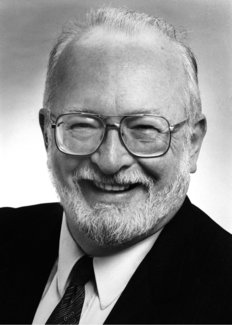
\includegraphics[height=0.36\linewidth]{figs/lauterbur-13686-content-portrait-mobile-tiny}
		}{\urlSource{https://is.gd/HgbMvo}}
		\label{subfig:paullauterbur}
	}
	\hspace{0.1\linewidth}
	\subfigure[تصویر هرمن کار]{
		\copyrightbox[b]{
		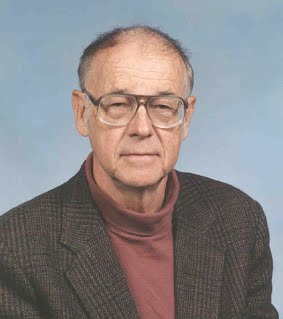
\includegraphics[height=0.36\linewidth]{figs/herman_carr}
		}{\urlSource{https://is.gd/teAHxS}}
		\label{subfig:herman-carr}
	}
	\hspace{0.1\linewidth}
	\subfigure[تصویر Peter-Mansfield]{
		\copyrightbox[b]{
			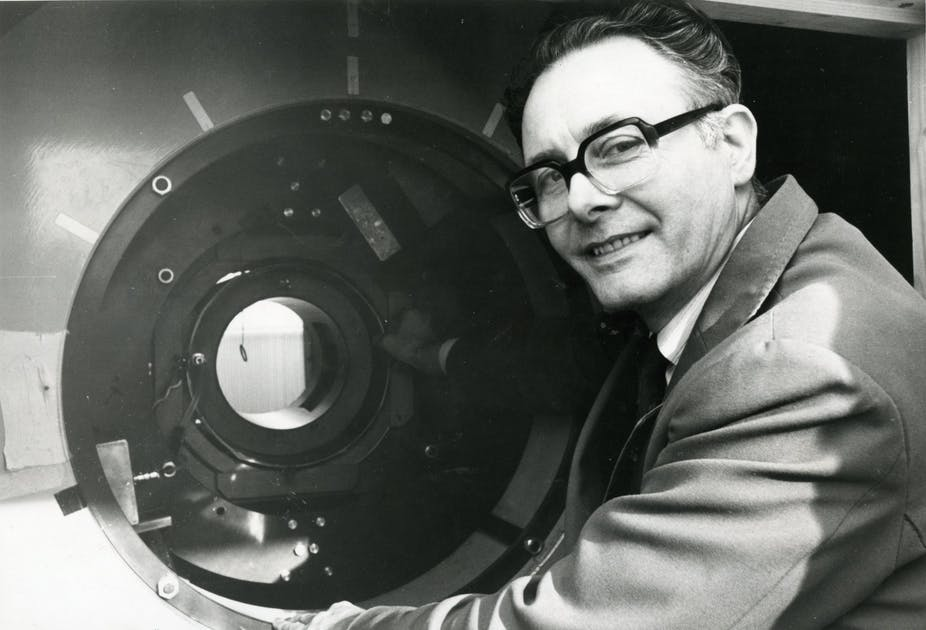
\includegraphics[height=0.36\linewidth]{figs/Peter-Mansfield}
		}{\urlSource{https://is.gd/W7AXIL}}
		\label{subfig:Peter-Mansfield}
	}


%	\end{minipage}
%	}{\scriptsize\url{https://www.nobelprize.org/prizes/medicine/2003/lauterbur/biographical/}
%		\url{https://sites.google.com/a/pbsd.k12.pa.us/magnetic-resonance-imaging/herman-carr}
%		\url{https://theconversation.com/obituary-professor-sir-peter-mansfield-whose-invention-of-the-mri-scanner-revolutionised-medicine-72815}}
	\caption{تصویر سازندگان اصلی دستگاه تصویربرداری \mri}
	
	
\end{figure}



\begin{figure}
	\centering
	\copyrightbox[b]{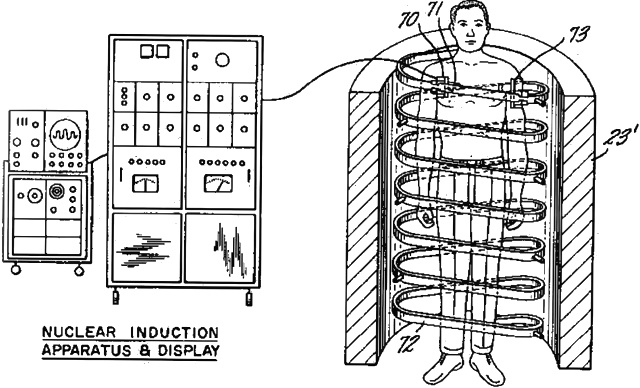
\includegraphics[width=0.6\linewidth]{figs/Damadian_invention}}
	{\urlSource{https://w.wiki/3STS}}
	\caption{تصویری از آرشیو اداره ثبت اختراعات آمریکا که متعلق به ریموند دامادیان، دانشمند آمریکایی و یکی از مخترعین سیستم‌های نوین ام آر آی}
	\label{fig:Damadian_invention}
\end{figure}


\subsection{بررسی مفهوم اسپین}
 

ساختار یک اتم، یک از اجزای اساسی در آزمایشات تشدید مغناطیسی است. اتم ها از سه ذره اصلی 
\LTRfootnote{Fundamental Particles}
تشکیلی شده اند:
\begin{enuminline}
	\item پروتون، که بار مثبت دارد
	\item نوترون، که بدون بار است
	\item الکترون، که بار الکتریکی منفی دارد
\end{enuminline}.
پروتون‌ها و نوترون‌ها در درون هسته اتم قرار گرفته اند و الکترون‌ها در خارج هسته به دور آن می‌گردند.
همچنین \textit{عدد‌اتمی}
\LTRfootnote{Atomic Number}
تعداد پروتون‌های یک اتم و \textit{جرم‌اتمی}
\LTRfootnote{Atomic Weight}
، تعداد پروتون‌ها و نوترون‌ها در یک اتم را نشان می‌دهد. اگر دو اتم عدد‌‌اتمی یکسان اما عدد جرمی متفاوت داشته باشند، آن دو اتم را \textit{همریخت} یا \textit{ایزوتوپ}
\LTRfootnote{Isotope}
یکدیگر می‌نامند. که خواص شیمیایی مشابهی اما با نرخ‌های متفاوت دارند.


\begin{figure}[t]
	\centering
	\subfigure[اسپین]{		
		\copyrightbox[b]{
			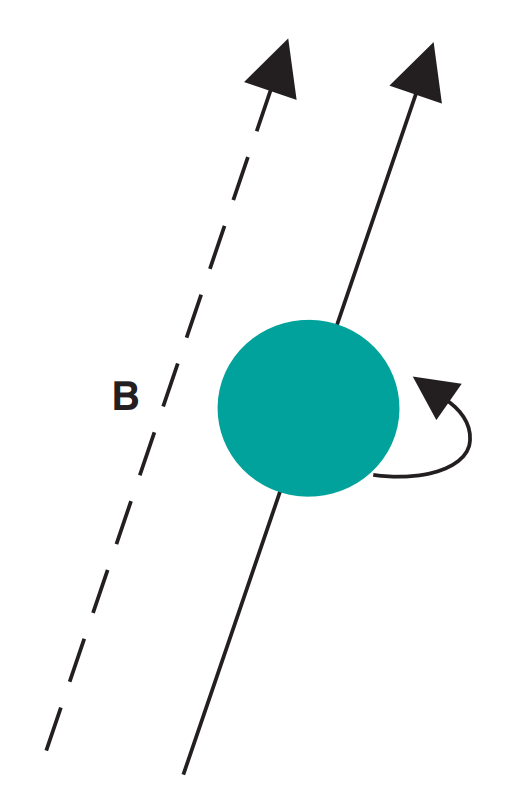
\includegraphics[height=0.3\linewidth]{figs/one-spin}
		}{\scriptsize\Doi{10.1002/9781119013068}}
		\label{fig:one-spin}}
		\hspace{0.2\linewidth}
	\subfigure[مغناطیس]{
		\copyrightbox[b]{
			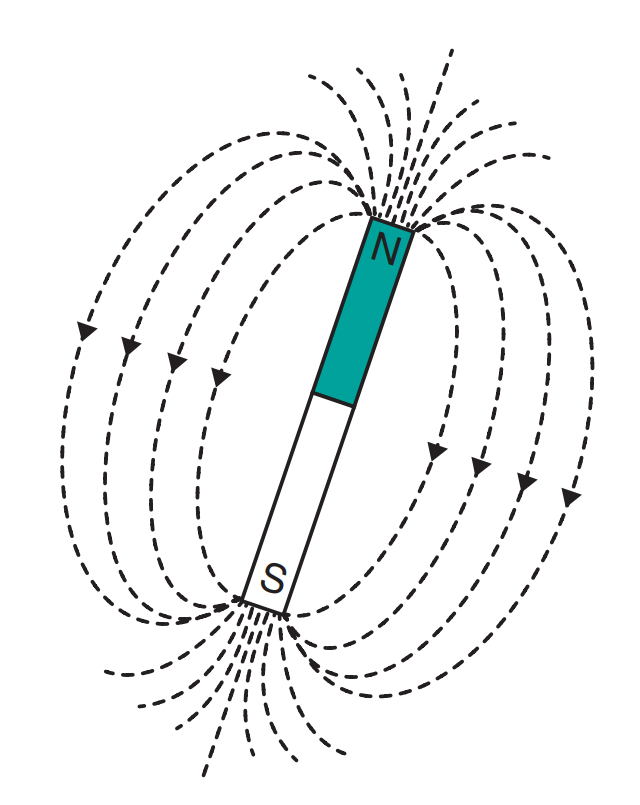
\includegraphics[height=0.3\linewidth]{figs/one-magnet}
		}{\scriptsize\Doi{10.1002/9781119013068}}
		\label{fig:one-magnet}}
	\caption{} 
\end{figure}

یکی دیگر از خواص هسته‌ها، اسپین
\index{اسپین}
\LTRfootnote{Spin}
یا اندازه حرکت زاویه ای ذاتی اسپینی
\LTRfootnote{Intrinsic Spin Angular Momentum}
است.
هسته هایی که حرکت اسپینی دارند همواره حول یک محور درحال گردش هستند.(شکل \ref{fig:one-spin} حرکت اسپینی را نمایش می‌دهد.)
تمام عناصر جدول تناوبی
\LTRfootnote{Periodic Table}
بجز آرگون
\LTRfootnote{Argon}
و سریم
\LTRfootnote{Cerium}
حداقل یک ایزوتوپ دارند که حرکت اسپینی دارد. از آنجا که این حرکت نقش مهمی در اصول تصویربرداری \mri دارد، بنابراین تقریبا تمامی عناصر قابلیت مشاهده شدن در تصویربرداری \mri را دارند. اسپین یکی از خواص کوانتومی هسته است و تعداد محدودی اسپین در طبیعت وجود دارند. 


\begin{table}[b]
	\centering
	\begin{tabular}{|c|c||C{10em}|}
		\hline \rowcolor{lightgray}
		
		تعداد پروتون & تعداد نوترون & عدد اسپین
		\\\hline\hline
		زوج & زوج & صفر \\\hline
		فرد & فرد & عدد صحیح \\\hline
		فرد & زوج & 
		\multirow{2}{*}{عدد صحیح و نصفی}
		\\\cline{0-1}
		زوج & فرد &
		\\\hline
	\end{tabular}
	\caption{بررسی عدد اسپین نسبت به تعداد پروتون‌ها و تعداد نوترون ها }
	\label{table:spin-even-odd}
\end{table}

اسپین که با نماد $I$ و یا $\Phi$ نمایش می‌دهند، مقدایر کوانتیده‌ای به خود می‌گیرد به طوری که می‌تواند صفر یا یک عدد صحیح (مثل $1$و $2$و $3$و ...) و یا یک عدد صحیح و نصفی (مثل $0.5$و $1.5$و $2.5$ و ...) باشد. 
بنابر \cite{book:basic-principles-and-applications}، می‌توان جدول 
\ref{table:spin-even-odd}
را استخراج نمود. درحقیقت اتم‌هایی با عدد اتمی یا جرم اتمی فرد دارای اسپین هستند و اگر هردو زوج باشند، نمی‌توان آن‌ها را در تصویربرداری \mri مطالعه نمود. 

در تصویر برداری \mri ما برروی هسته‌هایی متمرکز هستیم که اسپین آن‌ها \f12 است. به‌طور خاص  در تصویربرداری \mri، هسته اتم هیدروژن
\ce{^1_1H}
(فراوان‌ترین ایزوتوپ هیدروژن) و اتم کربن
\ce{^{13}_6C}
(ایزوتوپ کمیاب اما مفید در تصویربرداری) استفاده می‌شود.\cite{Handouts-NMRhandout.html}
توجه هم داریم که فراوان ترین ایزوتوپ کربن یعنی 
\ce{^{12}_6C}
فاقد اسپین است زیرا تعداد پروتون ها و نوتورون های آن هردو زوج هستند و بنابراین قابل بررسی در تصویربرداری  \mri نیستند. البته اتم های دیگری نیز مانند 
\ce{^19_9F}،
\ce{^23_11Na} و
\ce{^31_15P}
نیز در این تصویربرداری حائز اهمیت می‌باشند.

% READ THIS: http://iverson.cm.utexas.edu/courses/310N/Handouts/NMRhandout.html

اتم هیدروژن 
\ce{^1_1H}
از آن جهت بسیار اهمیت دارد که اولا ساختار بسیار ساده‌ای دارد (هسته آن از یک تک پروتون تشکیل شده است) و ثانیا در ساختمان اصلی آب 
\ce{H2O}
بکار رفته‌اند.
بدن هر‌انسان به طور میانگین، از 60 درصد آب تشکیل شده است. همچنین برخی ارگان های بدن حتی تا 90 درصد از آب ساخته شده‌اند. مغز و قلب انسان 73 درصد آب، ریه ها 83 درصد، پوست 64 درصد، ماهیچه‌ها و کلیه‌ها 79 درصد و استخوان ها 31 درصد آب را شامل می‌شوند.\cite{science-water-you-water-and-human-body}
از این رو، اتم هیدروژن نقش تعیین کننده ای دارد. دقت نیز داریم که اتم اکسیژن \ce{^16_8O} اسپینی ندارد و بنابراین نقشی در تصویربرداری \mri ندارد. از آنجایی که آب در بافت های نرم به میزان بیشتری وجود دارد، این نوع تصویر برداری عموما برای تصویربرداری از نواحی دارای بافت نرم مانند مغز مورد استفاده قرار می‌گیرد.

از آنجایی که درون هسته مشکل از پروتون هاست، بارالکتریکی هسته مثبت است. از این رو، در صورت حرکت دورانی حول محور دوران خود، یک میدان مغناطیسی هم‌راستا با همان محور دوران، ایجاد می‌کند. جون‌که مقدار اندازه اسپین هسته یک مقدار ثابت است این میدان مغناطیسی نیز اندازه ثابتی دارد. بنابراین برای ممان مغناطیسی هسته
\LTRfootnote{Nuclear Magnetic Moment} 
دو مولفه‌ی مقدار و جهت میدان مغناطیسی می‌توان تعریف کرد. به عبارت دیگر یک هسته دارای اسپین را می‌توان به صورت یک آهن‌ربای میکروسکوپیک ریز درنظر گرفت
(شکل \ref{fig:one-magnet}).
برای یک پروتون یا همان هسته ی \ce{^1_1H}، ممان مغناطیسی $\mu$ و تکانه زاویه‌ای اسپینی
\LTRfootnote{Spin Angular Momentum}$\Phi$
با یک ثابت تناسب $\gamma$ به صورت زیر به یک دیگر مرتبط می‌شوند.

\begin{equation}
	\mu = \gamma . \Phi
\end{equation}

که $\gamma$ در رابطه‌ی بالا نسبت ژایرومغناطیسی 
\LTRfootnote{Gyromagnetic Ratio}
نامیده می‌شود و واحد  $\frac{\gamma}{2\pi}$
را عموما برحسب (\lr{MHz/Tesla})

بیان می‌کنند.



\begin{figure}[t]
	\centering
	\copyrightbox[b]{
		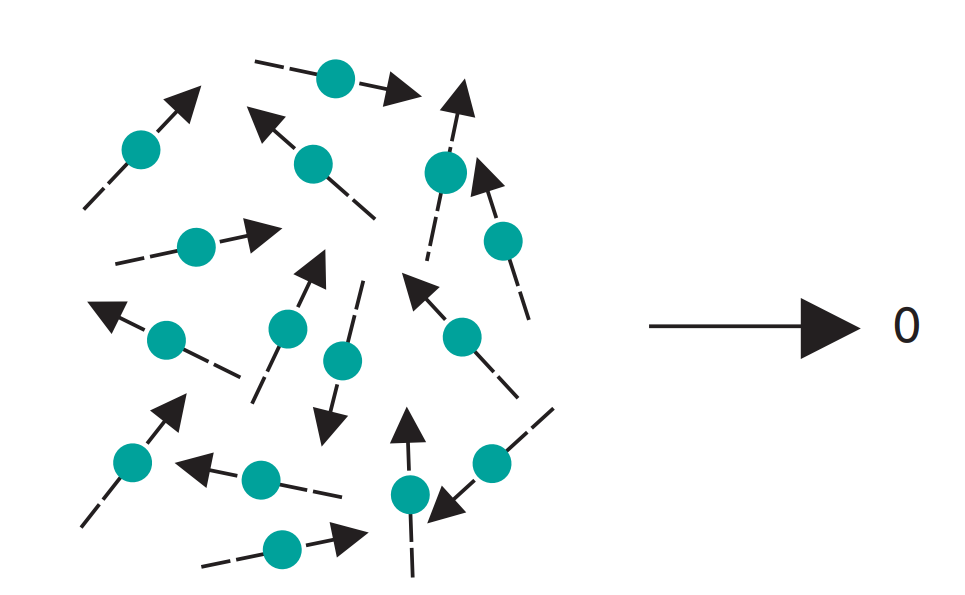
\includegraphics[width=0.5\linewidth]{figs/balance-spin}
	}{\scriptsize\Doi{10.1002/9781119013068}}
	\caption{}
	\label{fig:balance-spin}
\end{figure}


در اندازه گیری \mr مجموعه‌ای از این میدان های مغناطیسی کوچک مورد بررسی قرار می‌گیرد و به صورت تکی به قدری نیستند که بتوان آن‌ها را بررسی نمود. جهت این اسپین ها یک مکانیسم تصادفی دارد به طوری که در یک مجموعه هسته داری اسپین، در صورت عدم حضور میدان خارجی، برایند میدان مغناطیسی حاصل در آن مجمموعه صفر است و سیستم درحالت تعادل قرار دارد. 
(شکل \ref{fig:balance-spin}) در واقع تصاویر \mri در ابعاد ماکروسکوپیک ثبت می‌شوند.


\begin{figure}
	\centering
	\copyrightbox[b]{
		\centering
		\begin{minipage}{0.9\linewidth}
				\centering
				\subfigure[]{
				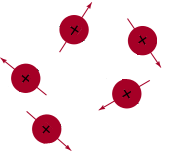
\includegraphics[height=0.25\linewidth]{mychapters/chapter-2/figs/alineamiento-no}	
				\label{subfig:alineamiento-no}}		
				\hspace{0.15\linewidth}
				\subfigure[]{
				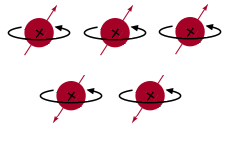
\includegraphics[height=0.22\linewidth]{mychapters/chapter-2/figs/alineamiento-yes}	
				\label{subfig:alineamiento-yes}} 
		\end{minipage}	
	}{\urlSource{http://www.qorganica.es/QOT/T12/alineamiento_e_exported/index.html}}
	\caption{}\label{fig:alineamiento}
\end{figure}



\begin{figure}
	\centering	
	\subfigure[]{
	\copyrightbox[b]{
		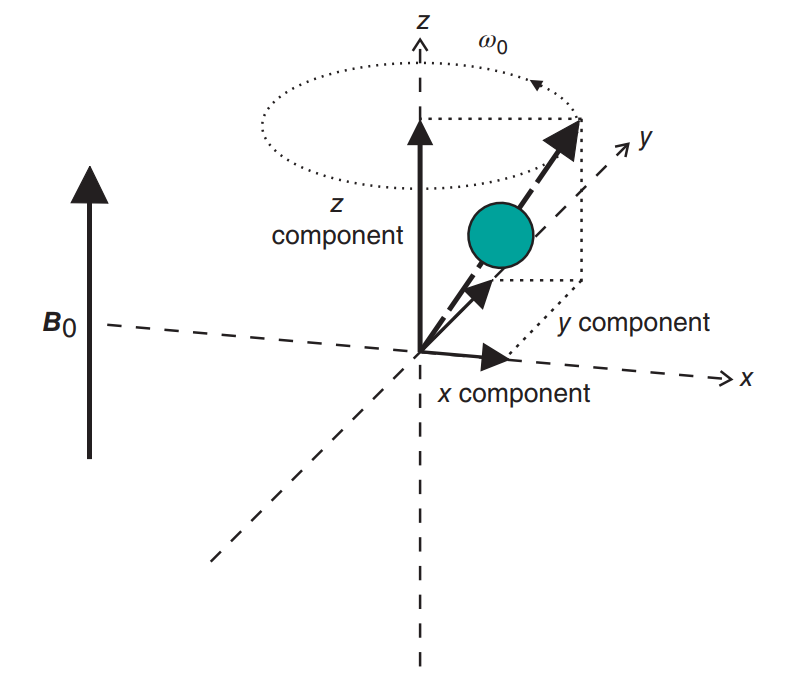
\includegraphics[height=0.35\linewidth]{figs/B-spin}	
		\label{subfig:precession-spin}
	}{\scriptsize\Doi{10.1002/9781119013068}}}
	\hspace{0.1\linewidth}
	\subfigure[]{
	\copyrightbox[b]{
		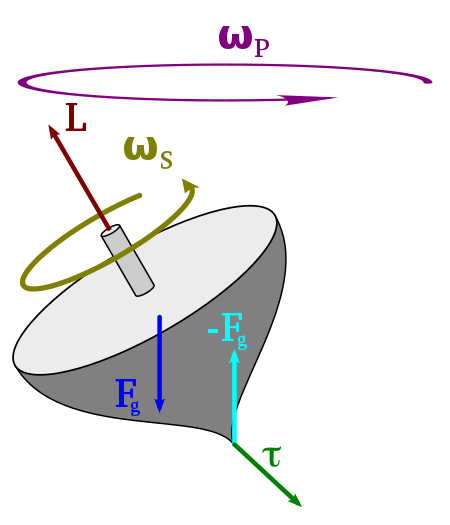
\includegraphics[height=0.3\linewidth]{mychapters/chapter-2/figs/PrecessionOfATop}	
		\label{subfig:precession-top}
	}{\urlSource{https://w.wiki/3TPJ}}}
	\caption{}
	\label{fig:precession}

\end{figure}

هنگامی که پورتون دارای اسپین در داخل یک میدان مغناطیسی قوی 
\RTLfootnote{
هنگامی که از میدان مغناطیسی قوی صحبت می‌کنیم منظور چیزی حدود حداقل $1$ تسلا یا $10000$ گاوس است. 
}
خارجی $B_0$ قرار می‌گیرند، اولا ممان های مغناطیسی اتم ها تمایل پیدا می‌کنند که در راستای یا خلاف راستای 
\LTRfootnote{Parallel or Anti-parallel}
قرار بگیرند (شکل \ref{subfig:alineamiento-yes} و ثانیا وادار می‌شوند که حرکت چرخشی حول راستای میدان مغناطیسی خارجی داشته باشند که به این پدیده حرکت تقدیمی
\LTRfootnote{Precession}
می‌گویند. 

\begin{figure}
	\centering
	\copyrightbox[b]{
	\begin{minipage}{\linewidth}\centering
	\subfigure[]{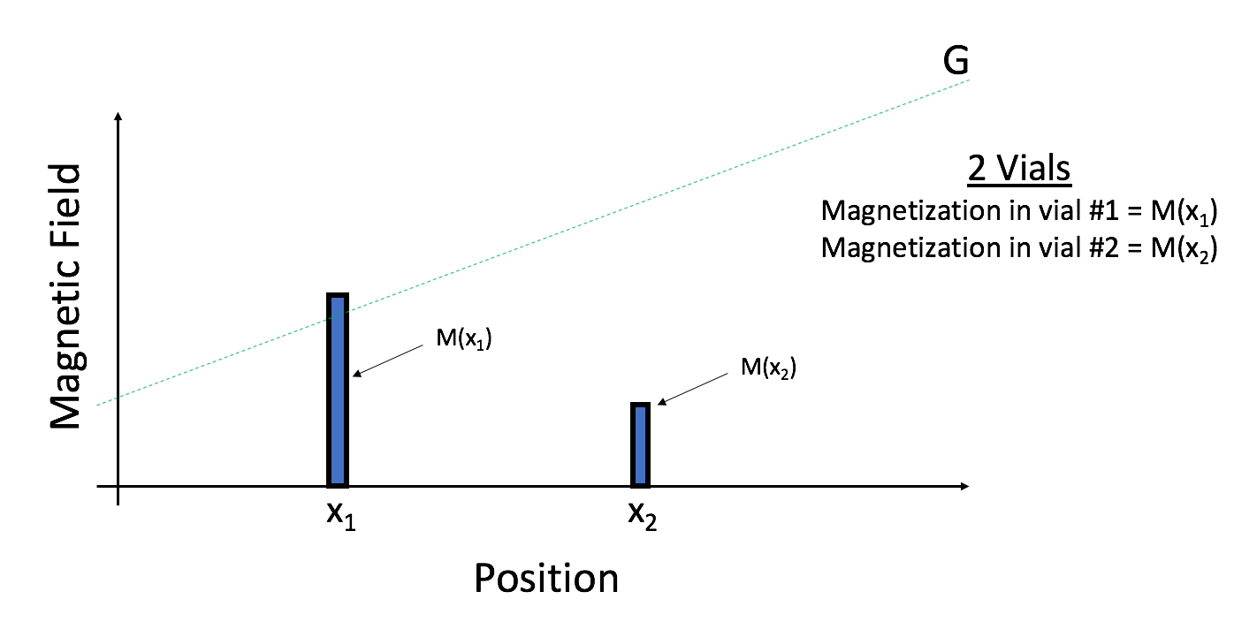
\includegraphics[height=0.23\linewidth]{figs/gr-1}\label{subfig:gr1}}
	\hspace{0.08\linewidth}
	\subfigure[]{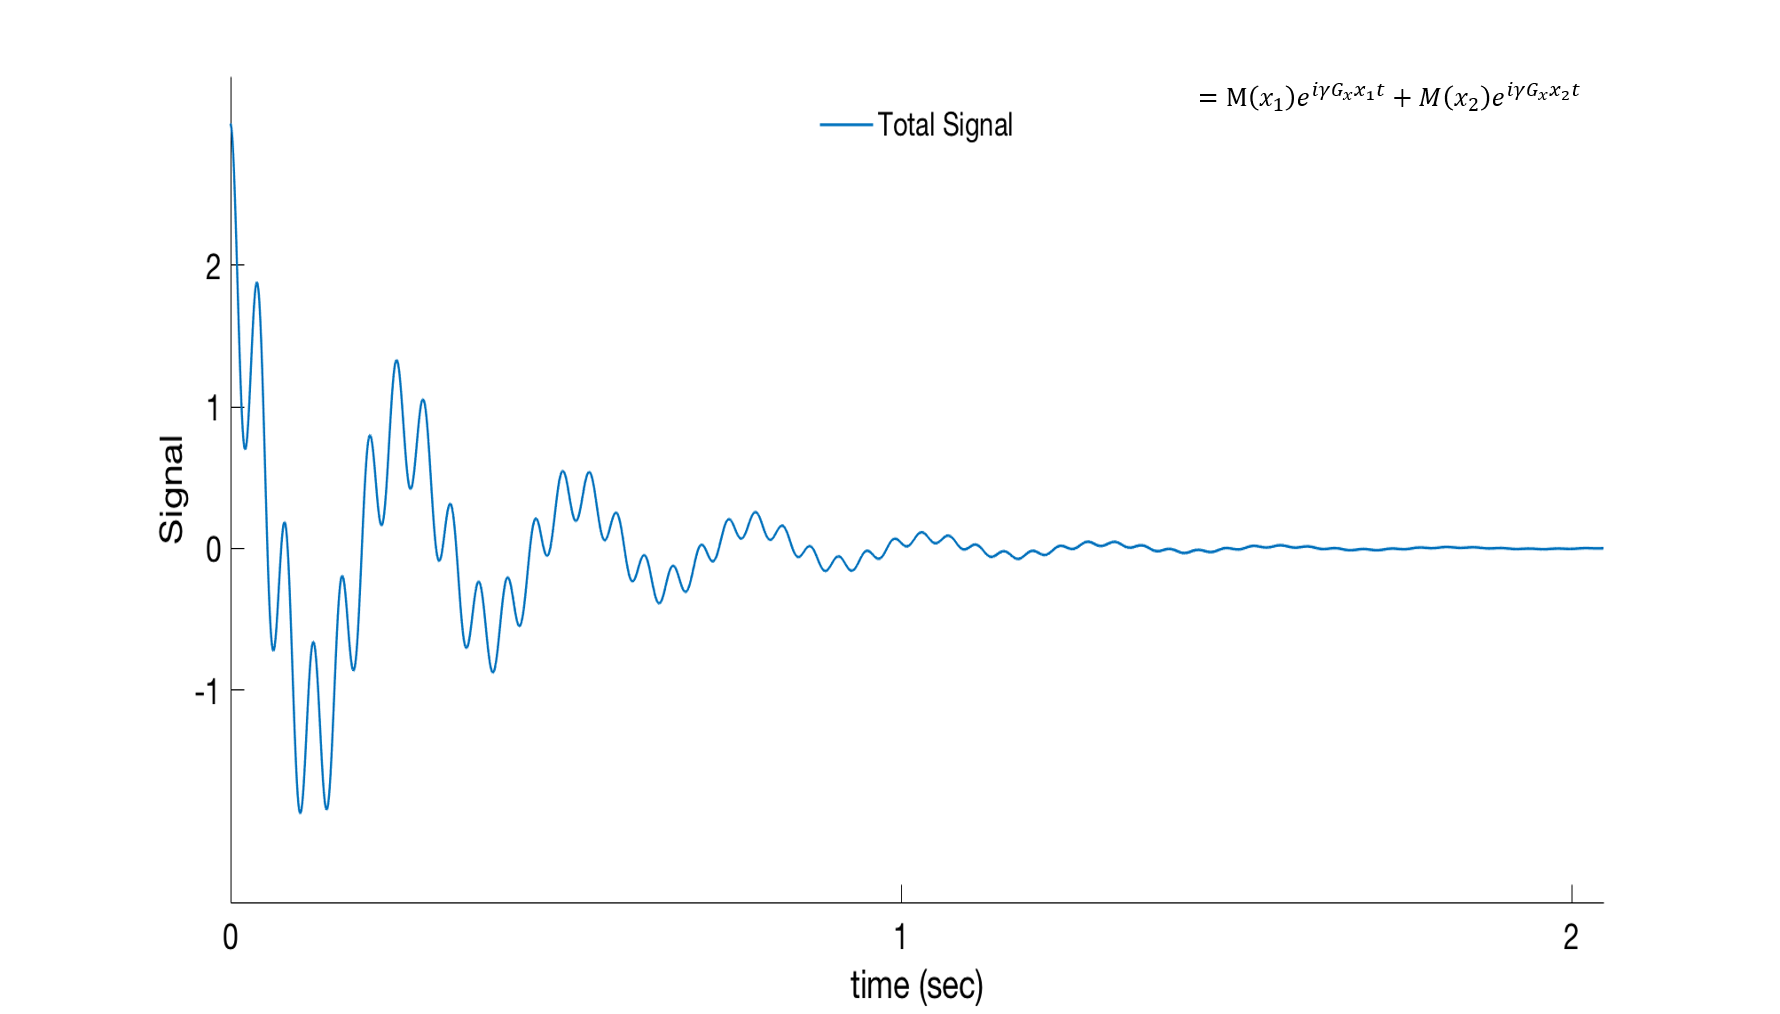
\includegraphics[height=0.23\linewidth]{figs/gr-3}\label{subfig:gr3}}
	\subfigure[]{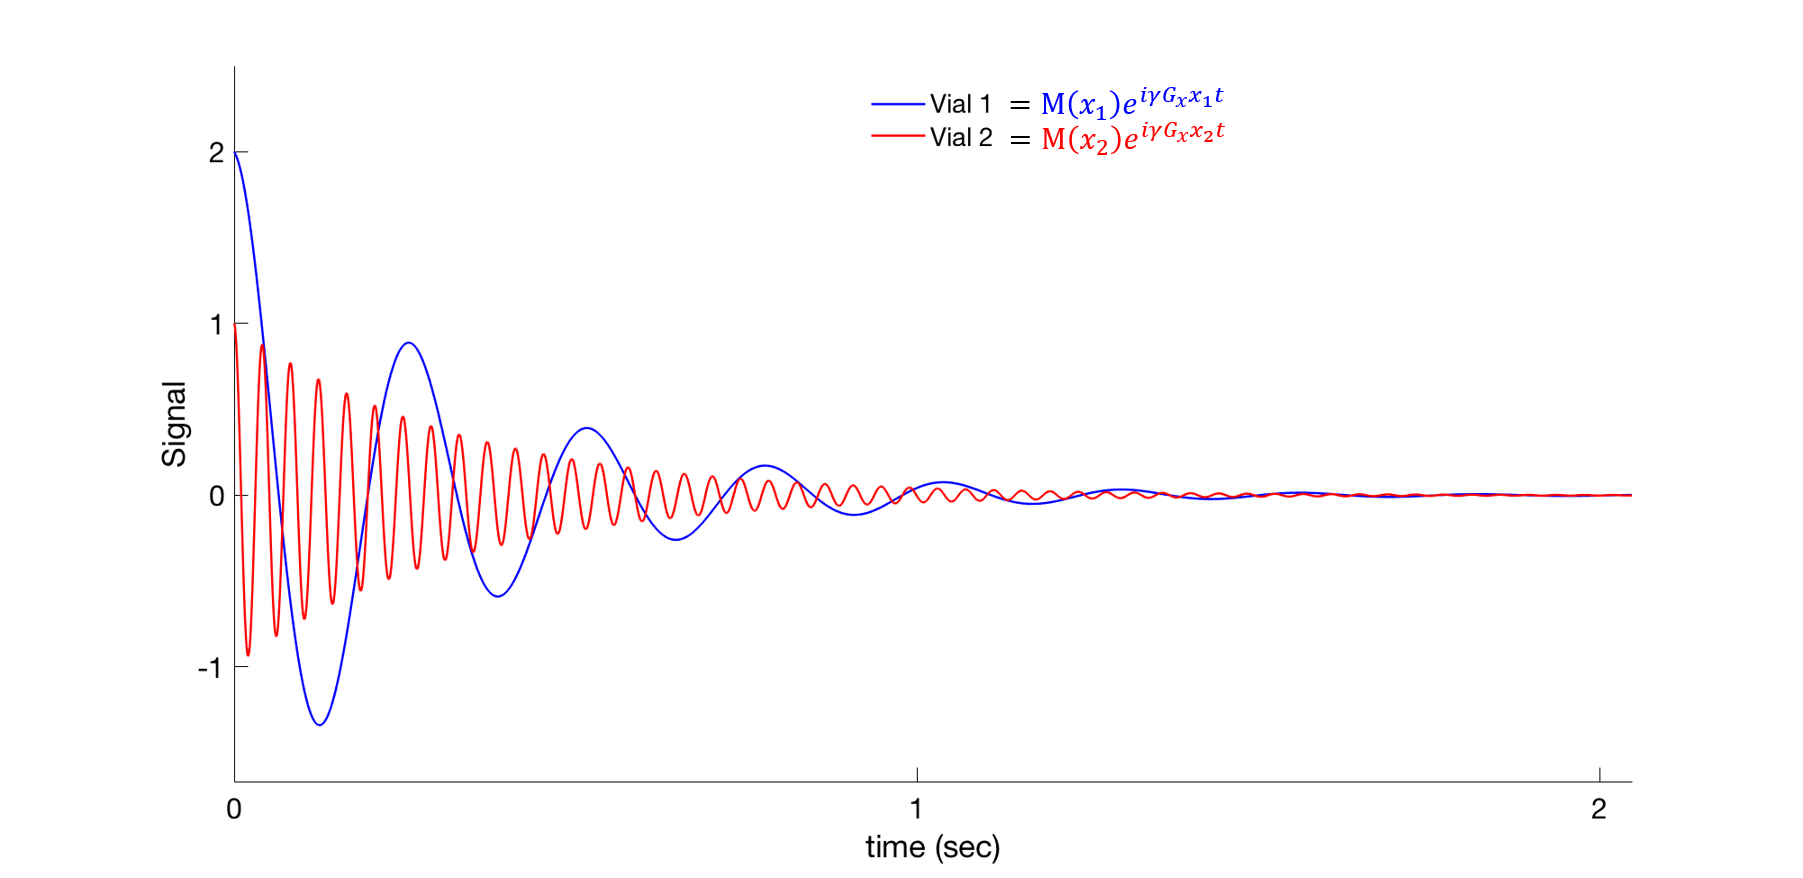
\includegraphics[height=0.23\linewidth]{figs/gr-2}\label{subfig:gr2}}
	\hspace{0.08\linewidth}
	\subfigure[]{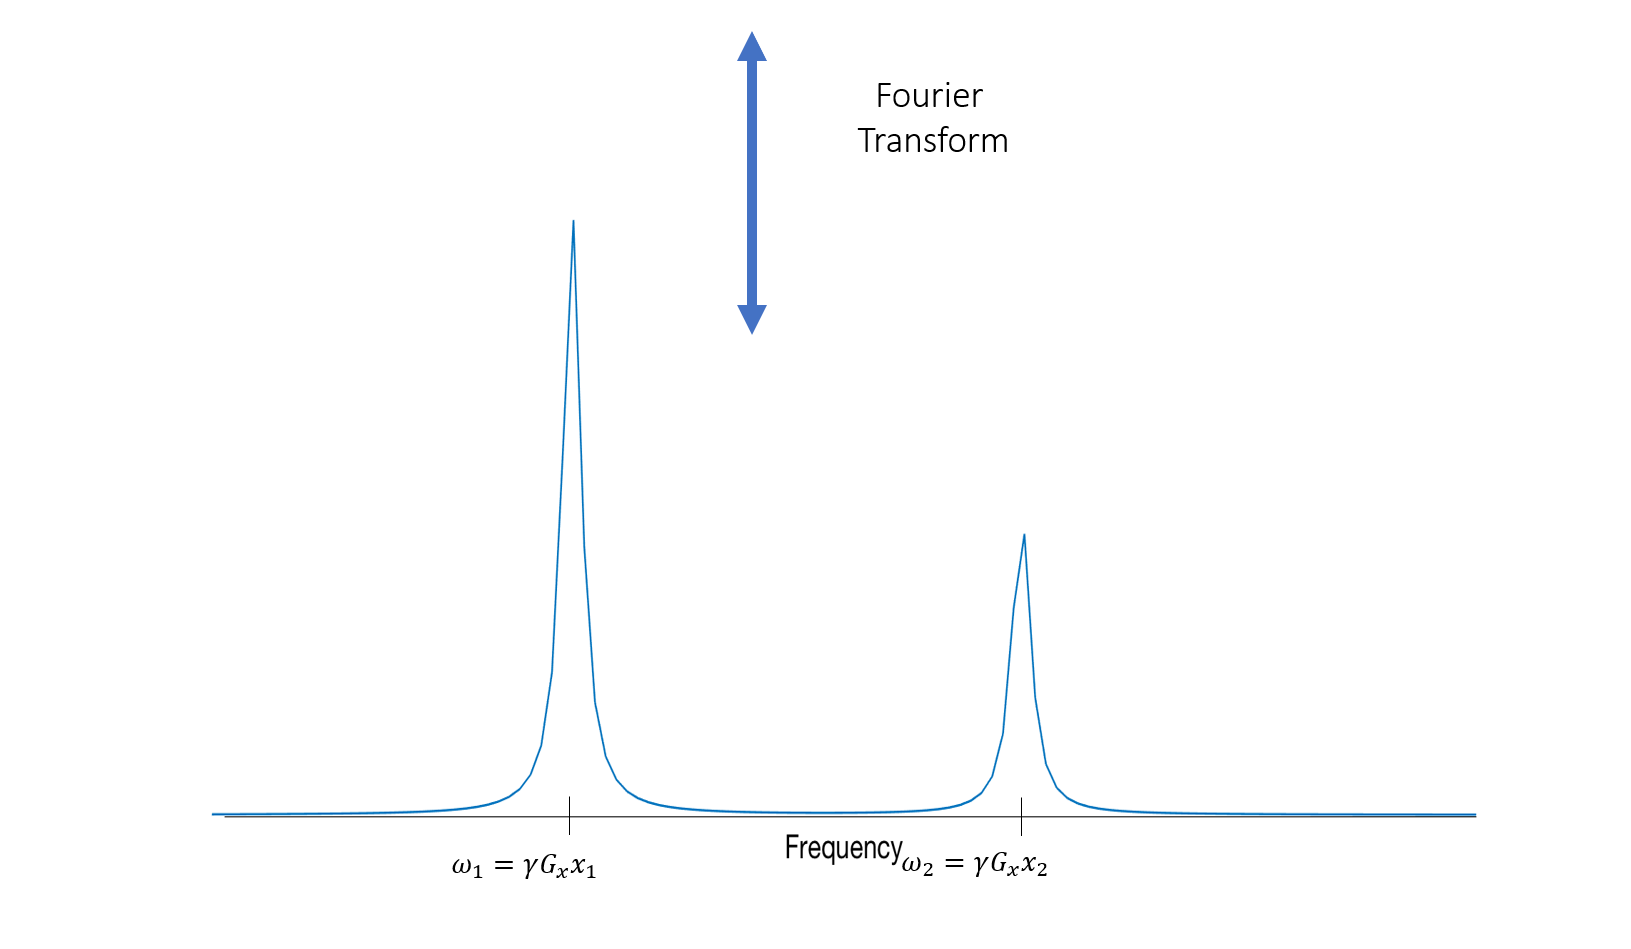
\includegraphics[height=0.25\linewidth]{figs/gr-4}\label{subfig:gr4}}
	\end{minipage}
	}{\urlSource{https://yout.be/vC82NeZmL-M}}
	\caption{}
	\label{fig:gr}
\end{figure}



\begin{figure}
	\centering
	\copyrightbox[b]{
		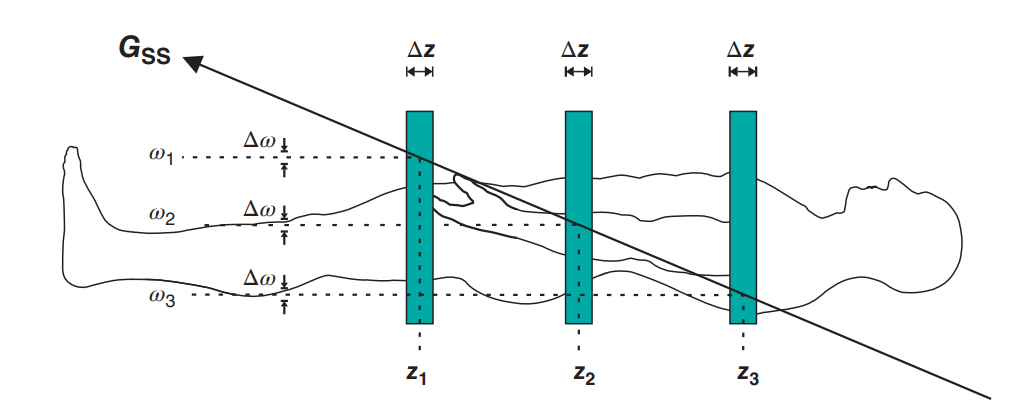
\includegraphics[width=0.7\linewidth]{figs/Slice-selection-process}
	}{\scriptsize\Doi{10.1002/9781119013068}}
	\caption{}
	\label{fig:slice-selection-process}
\end{figure}

\begin{figure}
	\centering
	\copyrightbox[b]{
		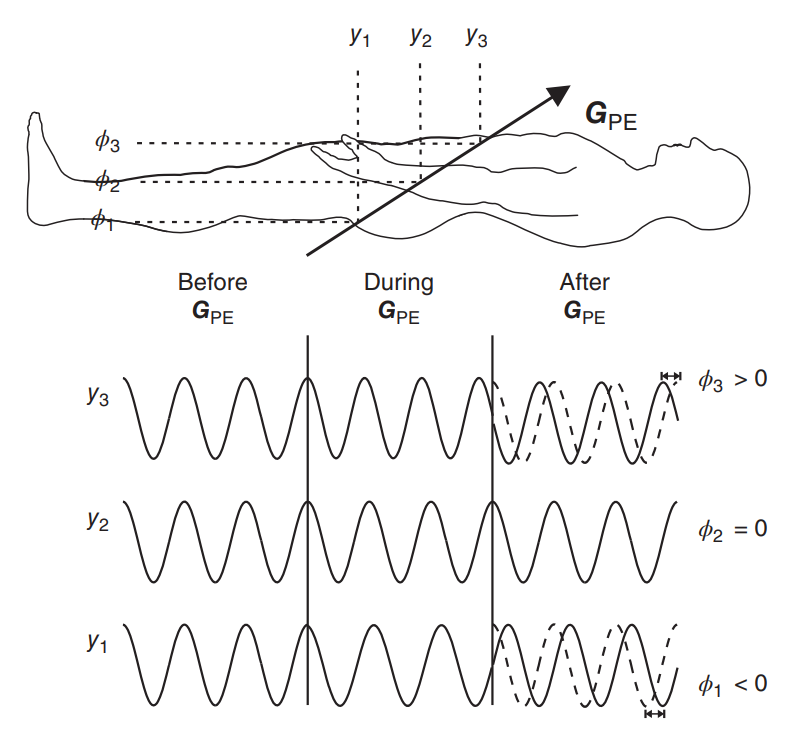
\includegraphics[width=0.7\linewidth]{figs/Concept-of-phase-encoding}
	}{\scriptsize\Doi{10.1002/9781119013068}}
	\caption{}
	\label{fig:concept-of-phase-encoding}
\end{figure}













